%% 
%% Copyright 2007, 2008, 2009 Elsevier Ltd
%% 
%% This file is part of the 'Elsarticle Bundle'.
%% ---------------------------------------------
%% 
%% It may be distributed under the conditions of the LaTeX Project Public
%% License, either version 1.2 of this license or (at your option) any
%% later version.  The latest version of this license is in
%%    http://www.latex-project.org/lppl.txt
%% and version 1.2 or later is part of all distributions of LaTeX
%% version 1999/12/01 or later.
%% 
%% The list of all files belonging to the 'Elsarticle Bundle' is
%% given in the file `manifest.txt'.
%% 
%% Template article for Elsevier's document class `elsarticle'
%% with harvard style bibliographic references
%% SP 2008/03/01

\documentclass[preprint,12pt,authoryear]{elsarticle}

%% Use the option review to obtain double line spacing
%% \documentclass[authoryear,preprint,review,12pt]{elsarticle}

%% Use the options 1p,twocolumn; 3p; 3p,twocolumn; 5p; or 5p,twocolumn
%% for a journal layout:
%% \documentclass[final,1p,times,authoryear]{elsarticle}
%% \documentclass[final,1p,times,twocolumn,authoryear]{elsarticle}
%% \documentclass[final,3p,times,authoryear]{elsarticle}
%% \documentclass[final,3p,times,twocolumn,authoryear]{elsarticle}
%% \documentclass[final,5p,times,authoryear]{elsarticle}
%% \documentclass[final,5p,times,twocolumn,authoryear]{elsarticle}

%% For including Fig.s, graphicx.sty has been loaded in
%% elsarticle.cls. If you prefer to use the old commands
%% please give \usepackage{epsfig}

%% The amssymb package provides various useful mathematical symbols
\usepackage{amssymb}
%% The amsthm package provides extended theorem environments
%% \usepackage{amsthm}
\usepackage{amsmath}

\usepackage[
  breaklinks=true,
  colorlinks=true,
  linkcolor=blue,anchorcolor=blue,
  citecolor=blue,filecolor=blue,
  menucolor=blue,pagecolor=blue,
  urlcolor=blue]{hyperref}

% Let's add todonotes and comments:
\usepackage[draft]{todonotes}

% Select what to do with command \comment:  
% \newcommand{\comment}[1]{}  %comment not showed
\newcommand{\comment}[1]
{{[\bfseries \color{blue} #1]}} %comment showed

%% The lineno packages adds line numbers. Start line numbering with
%% \begin{line numbers}, end it with \end{linenumbers}. Or switch it on
%% for the whole article with \linenumbers.
\usepackage{lineno}
\usepackage{float}
%\usepackage{wrapfig}
%\usepackage[backend=bibtex]{biblatex}  % to compile bib in R: http://texblog.org/2013/08/20/rknitr-automatic-bibliography-generation-with-biblatex-in-rstudio/


\begin{document}

\begin{frontmatter}

%% Title, authors and addresses

%% use the tnoteref command within \title for footnotes;
%% use the tnotetext command for theassociated footnote;
%% use the fnref command within \author or \address for footnotes;
%% use the fntext command for theassociated footnote;
%% use the corref command within \author for corresponding author footnotes;
%% use the cortext command for theassociated footnote;
%% use the ead command for the email address,
%% and the form \ead[url] for the home page:
%% \title{Title\tnoteref{label1}}
%% \tnotetext[label1]{}
%% \author{Name\corref{cor1}\fnref{label2}}
%% \ead{email address}
%% \ead[url]{home page}
%% \fntext[label2]{}
%% \cortext[cor1]{}
%% \address{Address\fnref{label3}}
%% \fntext[label3]{}

\title{DIYlandcover: Crowdsourcing the creation of systematic, accurate landcover maps}

%% use optional labels to link authors explicitly to addresses:
%% \author[label1,label2]{}
%% \address[label1]{}
%% \address[label2]{}

\author[label1,label2]{Estes, L.D.\corref{cor1} \fnref{fn1}}
\ead{lestes@princeton.edu}
\author[label3]{McRitchie, D.\fnref{fn1}}
\author[label1]{Choi, J.}
\author[label1]{Debats, S.}
\author[label4]{Evans, T.}
\author[label1]{Guthe, W.}
\author[label1]{Luo, D.}
\author[label1]{Ragazzo, G.}
\author[label1]{Zempleni, R.}
\author[label1]{Caylor, K.K.}

\address[label1]{Civil and Environmental Engineering, Princeton University, Princeton, NJ, 08544 USA}
\address[label2]{Woodrow Wilson School, Princeton University, Princeton, NJ, 08544 USA}
\address[label3]{Computational Science and Engineering Support, Office of Information Technology, Princeton University, Princeton, NJ, 08544 USA}
\address[label4]{Department of Geography, Indiana University, Bloomington, IN 47405 USA}
\cortext[cor1]{Corresponding author}
\fntext[fn1]{Equal contributors}

\begin{abstract}
% Abstract header text removed in elsearticle.cls to allow highlights to be inserted. 
\textbf{Highlights}
\begin{itemize}
  \item DIYlandcover crowdsources the generation of landcover data, using human pattern recognition skill to create accurate maps with rich geometric detail.  
  \item It incorporates systematic sampling and worker-specific accuracy assessment protocols, and connects to a large online job market. This design addresses three problems with crowdsourced mapping: representativity; data reliability; product delivery speed. 
  \item In a trial case, South African cropland was mapped with 91\% accuracy, and a large number of workers were recruited in a short time, suggesting rapid, but relatively expensive, map creation.
\end{itemize}
\textbf{Abstract}\\
Accurate landcover maps are fundamental to understanding socio-economic and environmental patterns and processes, but existing datasets contain substantial errors. Crowdsourcing map creation may substantially improve accuracy, but the quality and representativeness of crowdsourced data is hard to verify. We present an open-sourced platform, DIYlandcover, that systematically serves samples of high resolution imagery to an online job market, where workers delineate landcover features of interest. Worker mapping skill is frequently assessed, providing estimates of overall map accuracy and a basis for performance-based payments. An initial trial of DIYlandcover showed that novice workers delineated South African cropland with 91\% accuracy, which exceeds current generation global landcover products, while capturing important field geometry data. Given worker payment costs, large area, wall-to-wall mapping may be cost prohibitive, but a potentially promising use of DIYlandcover is to iteratively train and test emerging computer vision algorithms adapted for landcover mapping.   
\end{abstract}
%% Text of abstract

\begin{keyword}
remote sensing \sep landcover \sep crowd-sourcing \sep accuracy assessment \sep systematic sampling
\end{keyword}


\end{frontmatter}


\linenumbers

\section*{Availability}
\indent Anyone interested in applying DIYlandcover for non-commercial purposes may contact the authors for access to the source code. See \\ \href{http://mappingafrica.princeton.edu}{http://mappingafrica.princeton.edu} for further details regarding a specific application of this software.

%% main text
\section{Introduction}
Regional maps of landcover provide critical information on food security estimates \citep[e.g.][]{monfreda_farming_2008,licker_mind_2010,see_improved_2015,lobell_use_2013}, models of land-atmosphere interactions \citep[e.g.][]{liang_simple_1994}, and calculations of carbon stocks \citep[e.g.][]{ruesch_new_2008}, greenhouse gas emissions \citep[e.g.][]{searchinger_high_2015}, and habitat change \citep[e.g.][]{gibbs_tropical_2010}. These maps are particularly important in developing regions, such as sub-Saharan Africa, where government land use data are often lacking, error-prone, and inconsistent \citep{ramankutty_farming_2008,see_improved_2015}. These developing regions are also experiencing rapid land use changes \citep{gibbs_tropical_2010,rulli_global_2013} that pose pressing development challenges \citep[e.g. how to feed people at substantially lower environmental cost][]{searchinger_high_2015}. 

Unfortunately, landcover datasets derived from medium to coarse resolution satellite sensors are particularly inaccurate \citep{fritz_comparison_2010, fritz_identifying_2008}. One major reason for  poor accuracy is the fact that land use patterns in these regions are dominated by smallholder farming. Smallholder fields are typically smaller ($\leq$2 ha) than the resolution ($\sim$6 ha) of the most commonly used satellite imagery \citep{jain_mapping_2013}. Furthermore, smallholders often plant diverse mixtures of crops, which further increases within-pixel heterogeneity \citep{jain_mapping_2013}, and their fields often contain remnant trees and have irregular boundaries, which makes them spectrally harder to distinguish from the surrounding vegetation \citep{see_improved_2015, lobell_use_2013}. 

New techniques for merging multiple landcover products that incorporate expert ranking of cover classification are helping to substantially improve map accuracy \citep{fritz_cropland_2011,fritz_mapping_2015}. However, these approaches cannot overcome the mismatch between sensor resolution and smallholder field size. High resolution satellite imagery ($<$5 m) is becoming increasingly available--and presumably will become more affordable--so the resolution problem should be resolved in the near future \citep{see_improved_2015, lobell_use_2013}. However, high resolution comes at the cost of low frequency; a meter-scale dataset covering wide areas is necessarily pieced together using imagery acquired on different dates, by different sensors, pointing at different viewing angles. This resulting image quilt contains large and uncorrectable spectral variability caused by atmospheric effects, vegetation phenology, and even land use change. This variability propagates into classification error.  

It remains a major challenge to develop algorithms that can accurately map landcover in the face of both increased image variability and substantial spatial heterogeneity. Two possibilities have emerged: A first approach draws on  advances in computer vision and machine learning, using semantic segmentation \citep[e.g.][]{schroff_object_2008} and Randomized Quasi-Exhaustive feature selection \citep{tokarczyk_features_2015} to find optimal classifiers within highly variable smallholder fields \citep{debats_generalized_????}. A second approach is to employ humans, who are very adept at recognizing patterns in noisy images \citep{biederman_recognition-by-components:_1987}. The superiority of human over machine pattern recognition provides the motivation for CAPTCHA \citep{ahn_captcha:_2003}, which secures websites by requiring human users to recognize fuzzy or irregular letters and numbers that are too difficult for automated algorithms to identify. Human-interpreted landcover maps are thus likely to be consistently more accurate than automated classifiers. Unfortunately, since humans are much slower at data processing than computers, human-generated landcover maps covering large areas will require much more time and expense to create. However, this problem is being alleviated by the growth of the internet, which makes it increasingly feasible to turn pattern recognition problems into many small tasks that are undertaken by a large number of online workers---the human equivalent of parallel processing. This ability to ``crowdsource'' \citep{howe_rise_2006} such work supports projects ranging from galactic classification \citep{lintott_galaxy_2008} to ornithological surveys \citep{sullivan_ebird:_2009}. Crowdsourcing of landcover is already being used in the Geo-wiki project, which uses online volunteers to correct landcover data based on their own interpretations of high resolution satellite imagery \citep{fritz_geo-wiki.org:_2009, fritz_geo-wiki:_2012, fritz_mapping_2015}. Recently, these data have been used to create the most accurate (82\%) global cropland map \citep{fritz_cropland_2011, fritz_mapping_2015}.  

While the use of crowdsourcing is an extremely promising development for landcover mapping, many existing projects   (e.g. OpenStreetMap \href{openstreetmap.org}{(openstreetmap.org)}) are geared towards users who create content according to their personal interests, thus the resulting maps are unlikely to be geographically representative. Furthermore, verifying the accuracy of crowdsourced data is a challenge \citep{allahbakhsh_quality_2013, flanagin_credibility_2008, see_improved_2015} that remains largely unaddressed by existing platforms. In terms of using crowdsourcing to improve accuracy, prior efforts have focused primarily on validating pixel-based classifications, and less on delineating individual landcover objects, despite the fact that landcover geometry defines critical social and environmental characteristics of the land system \citep{fritz_mapping_2015}, and provide an important constraint for monitoring agroecosystems \citep[e.g][]{estes_projected_2013, estes_comparing_2013}. For example, field boundaries have been used as a filter to extract ``pure'', crop-specific time series of vegetation indices from MODIS imagery, allowing field-scale yield proxies to be derived \citep{estes_projected_2013, estes_comparing_2013}.  

In this paper, we describe \emph{\textbf{DIYlandcover}}, a new platform for creating crowdsourced landcover data that addresses the three aforementioned limitations. Specifically, our platform provides online workers with tools to 1) delineate landcover objects within 2) systematically selected locations, while the resulting maps are subjected to 3) periodic quality assessment, providing estimates of individual worker and overall map accuracy. We provide an overview of the DIYlandcover's design and mechanics, and report on the results of a trial application mapping crop fields in South Africa, which suggests that DIYlandcover allows inexperienced online workers to generate high accuracy ($>$90\%), geometrically rich, and geographically representative landcover data at a rate that may be  comparable to automated classification, when factoring in pre-processing and algorithm development time. 

\section{System design}
The inspiration for DIYlandcover came from GeoTerraImage, a company that mapped South Africa's arable cropland by manually digitizing fields visible in high resolution satellite imagery  \citep{geoterraimage_south_2008}. The resulting map set is 97\% accurate in distinguishing cropped from uncropped areas at a 1 km resolution (unpublished data), and provides rich detail on field type and geometry. However, making these maps was an expensive and lengthy process; given image purchase costs and hours for the staff members involved, the estimated cost was \$5 km$^{-2}$ (Ferreira, pers. comm.). 

We developed DIYlandcover to overcome these constraints of cost and production time, while retaining the advantages of human image interpretation skill demonstrated by GeoTerraImage. Our platform connects workers in an online job marketplace to a map application programming interface (API) that hosts high resolution satellite imagery. DIYlandcover currently works with Amazon's Mechanical Turk \citep{amazon_web_services_amazon_2012} and the Google Maps API, but these could in principle be replaced by other services. These two aspects of DIYlandcover substantially reduce both mapping costs and completion times, because the imagery is free and the platform can access a potentially large number of workers. 

Given the distributed and anonymous nature of the online job market, we cannot intensively train workers (as GeoTerraImage did), yet our mapping task is complex, requires significant image interpretation skill, and must be completed in a systematic manner. Therefore, to ensure the scientific quality of its maps, DIYlandcover incorporates site selection and accuracy assessment protocols (Fig. 1). A sampling grid (SG in Fig. 1) over the desired study region provides the basis for collecting stratified random samples. The first draw identifies sites where the researcher/administrator \citep[the ``Requester'';][]{allahbakhsh_quality_2013} will provide landcover reference maps (black cells). Subsequent draws select sites where workers will create new maps (grey cells). This sample of locations is then sent to the job marketplace. All workers must pass an initial qualification test (Q1 in Fig. 1) that proves their ability to map a handful of sites with a minimum level of skill. Once qualified, workers begin mapping. Each worker will map both grey and black sites, which are respectively referred to as N (for normal) and Q (for quality assessment) sites. Q sites are indistinguishable from N sites, and are intermingled such that each worker has a Requester-defined probability of encountering a Q site. Completed maps from N sites are inserted into DIYlandcover's database (D), while maps from Q sites are first scored according to their agreement with their reference maps (Q2 in Fig. 1). Maps that fall below a minimum score are rejected. Map scores are incorporated into a worker-specific quality score, which is used to assign confidence to all maps generated by a worker, and to determine overall map accuracy. Workers are paid (P in Fig. 1) for each site mapped, with the possibility of bonus payments linked to quality scores.    

\begin{figure}[!ht]
  \begin{center}
    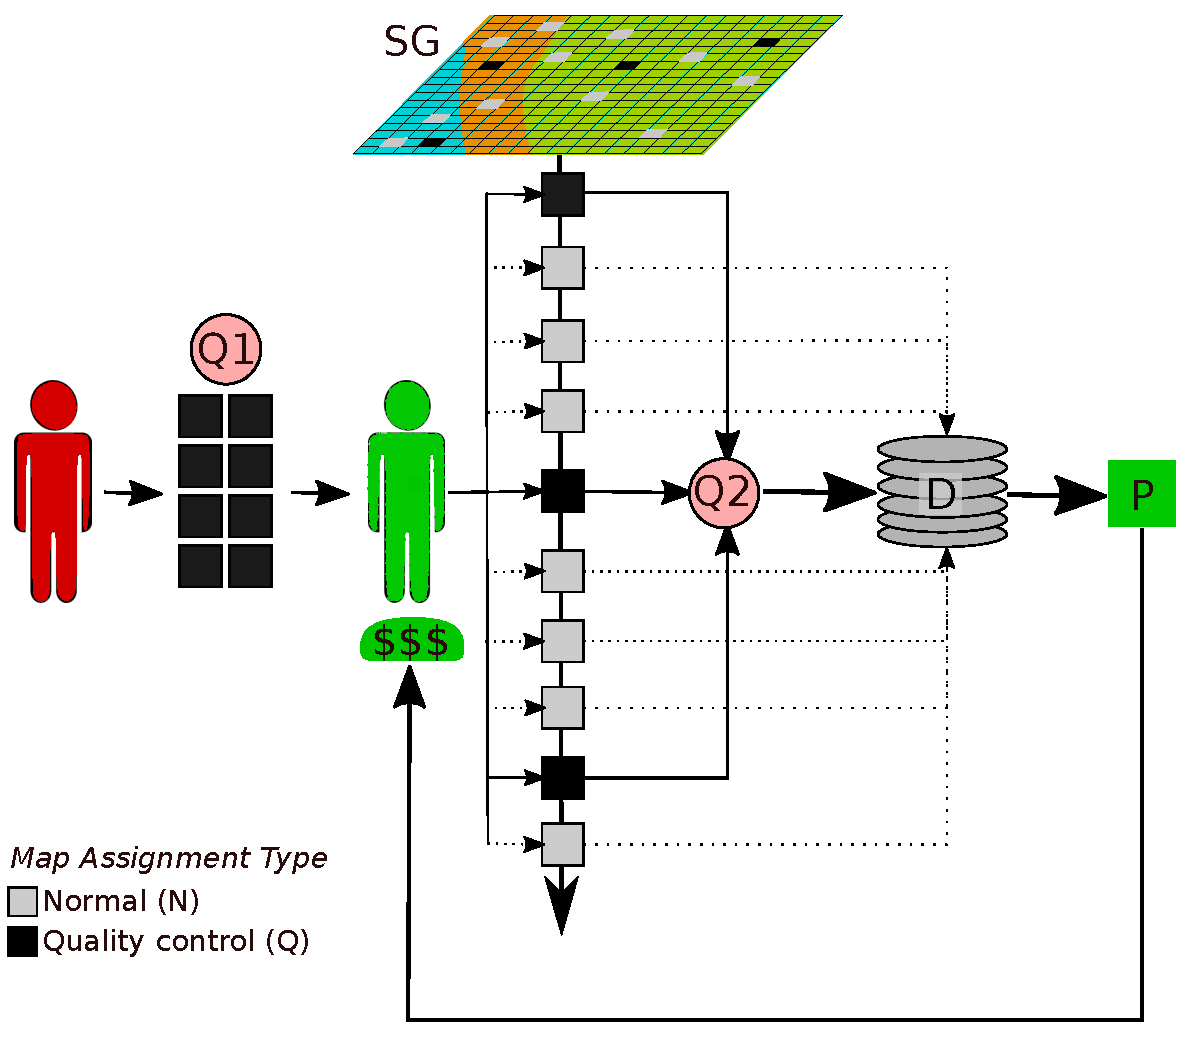
\includegraphics[scale=0.6]{figures/fig1.pdf}
    \caption{An overview of DIYlandcover's design. A survey grid (SG) is overlaid on a geographic area, and then random samples (weighted proportionally to the probability of cover type presence, represented by green, orange, and blue) are drawn to specify where groundtruth maps will be generated (black cells) to support worker map quality (Q) assessment. Subsequent random draws (grey cells) select sites that are undertaken as normal (N) mapping assignments. N and Q sites are sent inter-mingled to the online job marketplace for mapping. A first time worker (red) must take an initial map qualification test (Q1), after which she or he is qualified (green) and begins mapping. Maps from N sites are stored in the database (D); Q site maps are first scored based on their agreement with groundtruth (Q2). This score contributes to a longer term worker quality score, which is used to assess overall map quality and allows performance-based bonuses to be paid on of fixed per site payments (P).}
    \label{default}
  \end{center}
\end{figure}

\section{The mechanics of DIYlandcover}
The basic structure of DIYlandcover consists of three elements (Fig. 2): the main server hosting DIYlandcover's  database, here a Linux virtual machine with PostgresSQL (9.4) with the PostGIS (2.1) spatial extension;  a map server hosting the satellite imagery, in this case the Google Maps API \citep{google_developers_google_2012}; the online job market, Mechanical Turk \citep{amazon_web_services_amazon_2012}. Within this structure several key processes govern the creation and management of mapping tasks.  

\subsection{Site selection}
A ``master grid'' covering the study area is first created as a PostGIS table. Each cell provides a unique identifier, and the cell resolution defines the area of an individual mapping task. This grid is intersected with a second grid containing landcover occurrence probabilities, which are converted into categorical weights. A third field is created that indicates whether each cell is available to be mapped or not.  

%We use R \citep{r_development_core_team_r:_2011} and the raster \citep{etten_raster:_2011}, rgdal \citep{keitt_rgdal:_2012,warmerdam_geospatial_2008}, and rgeos \citep{bivand_rgeos:_2012} packages to generate the sampling grid, and then import it together with the probability grid into PostGIS where the intersection operations are performed.  

\begin{figure}[!ht]
  \begin{center}
       \makebox[\textwidth][c]{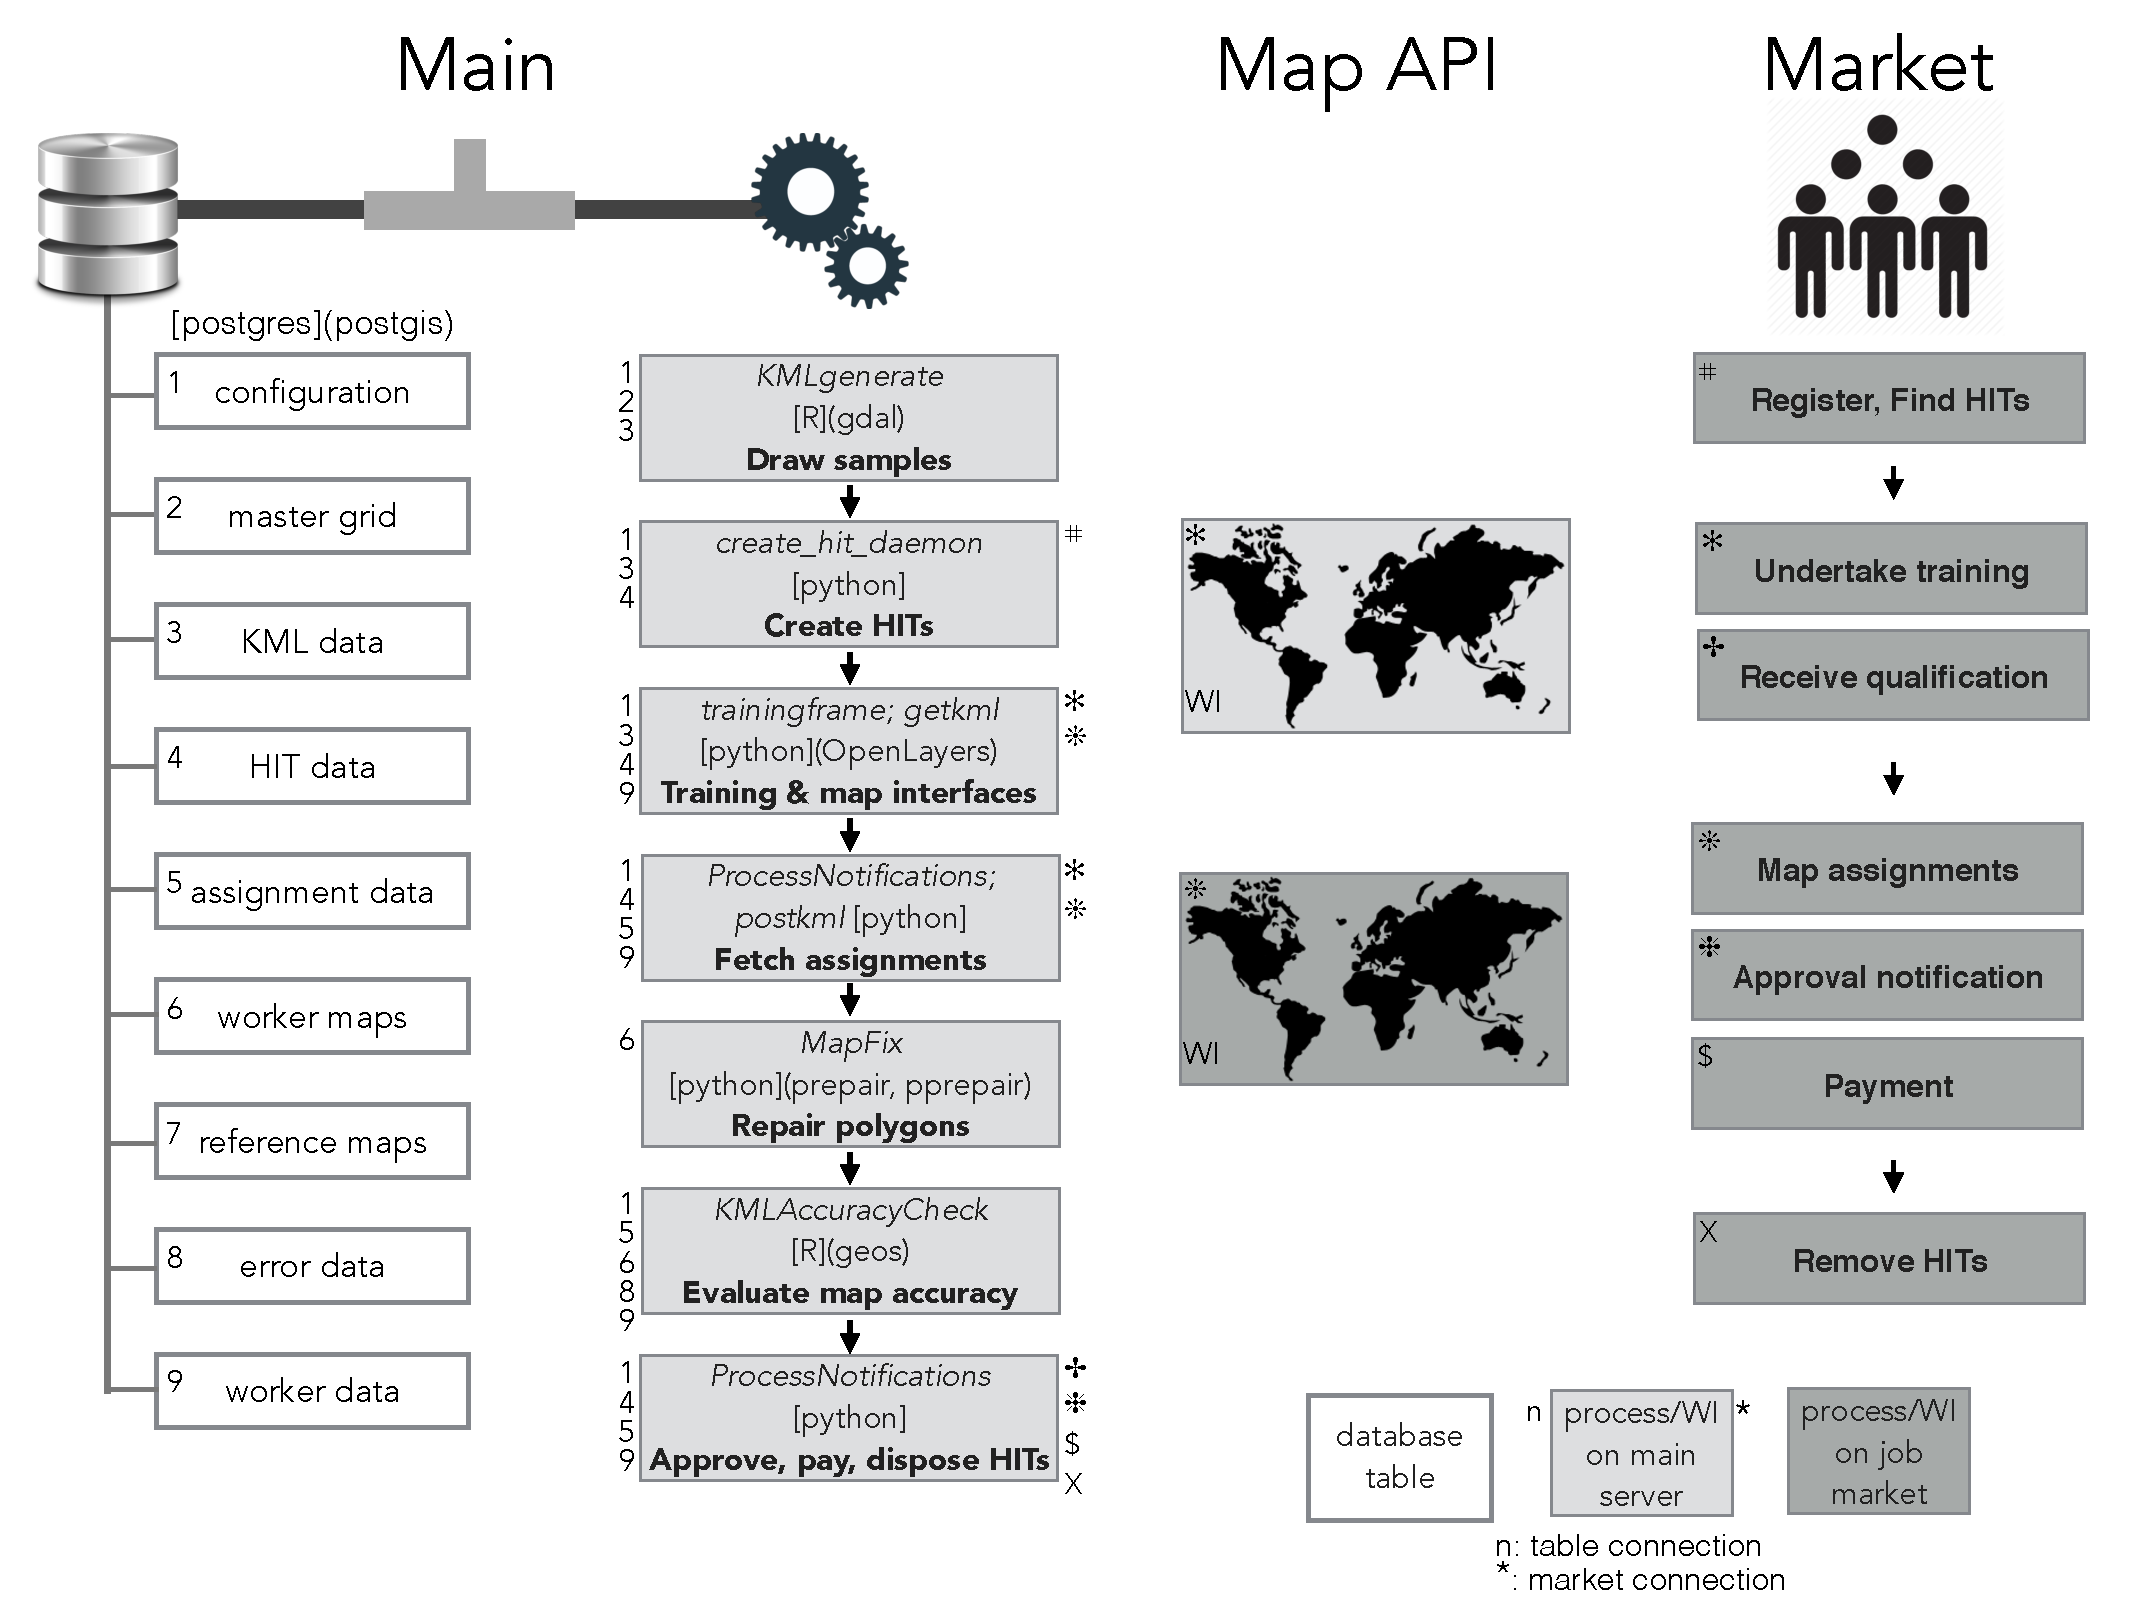
\includegraphics[width=1.3\textwidth]{figures/fig2.pdf}}
    %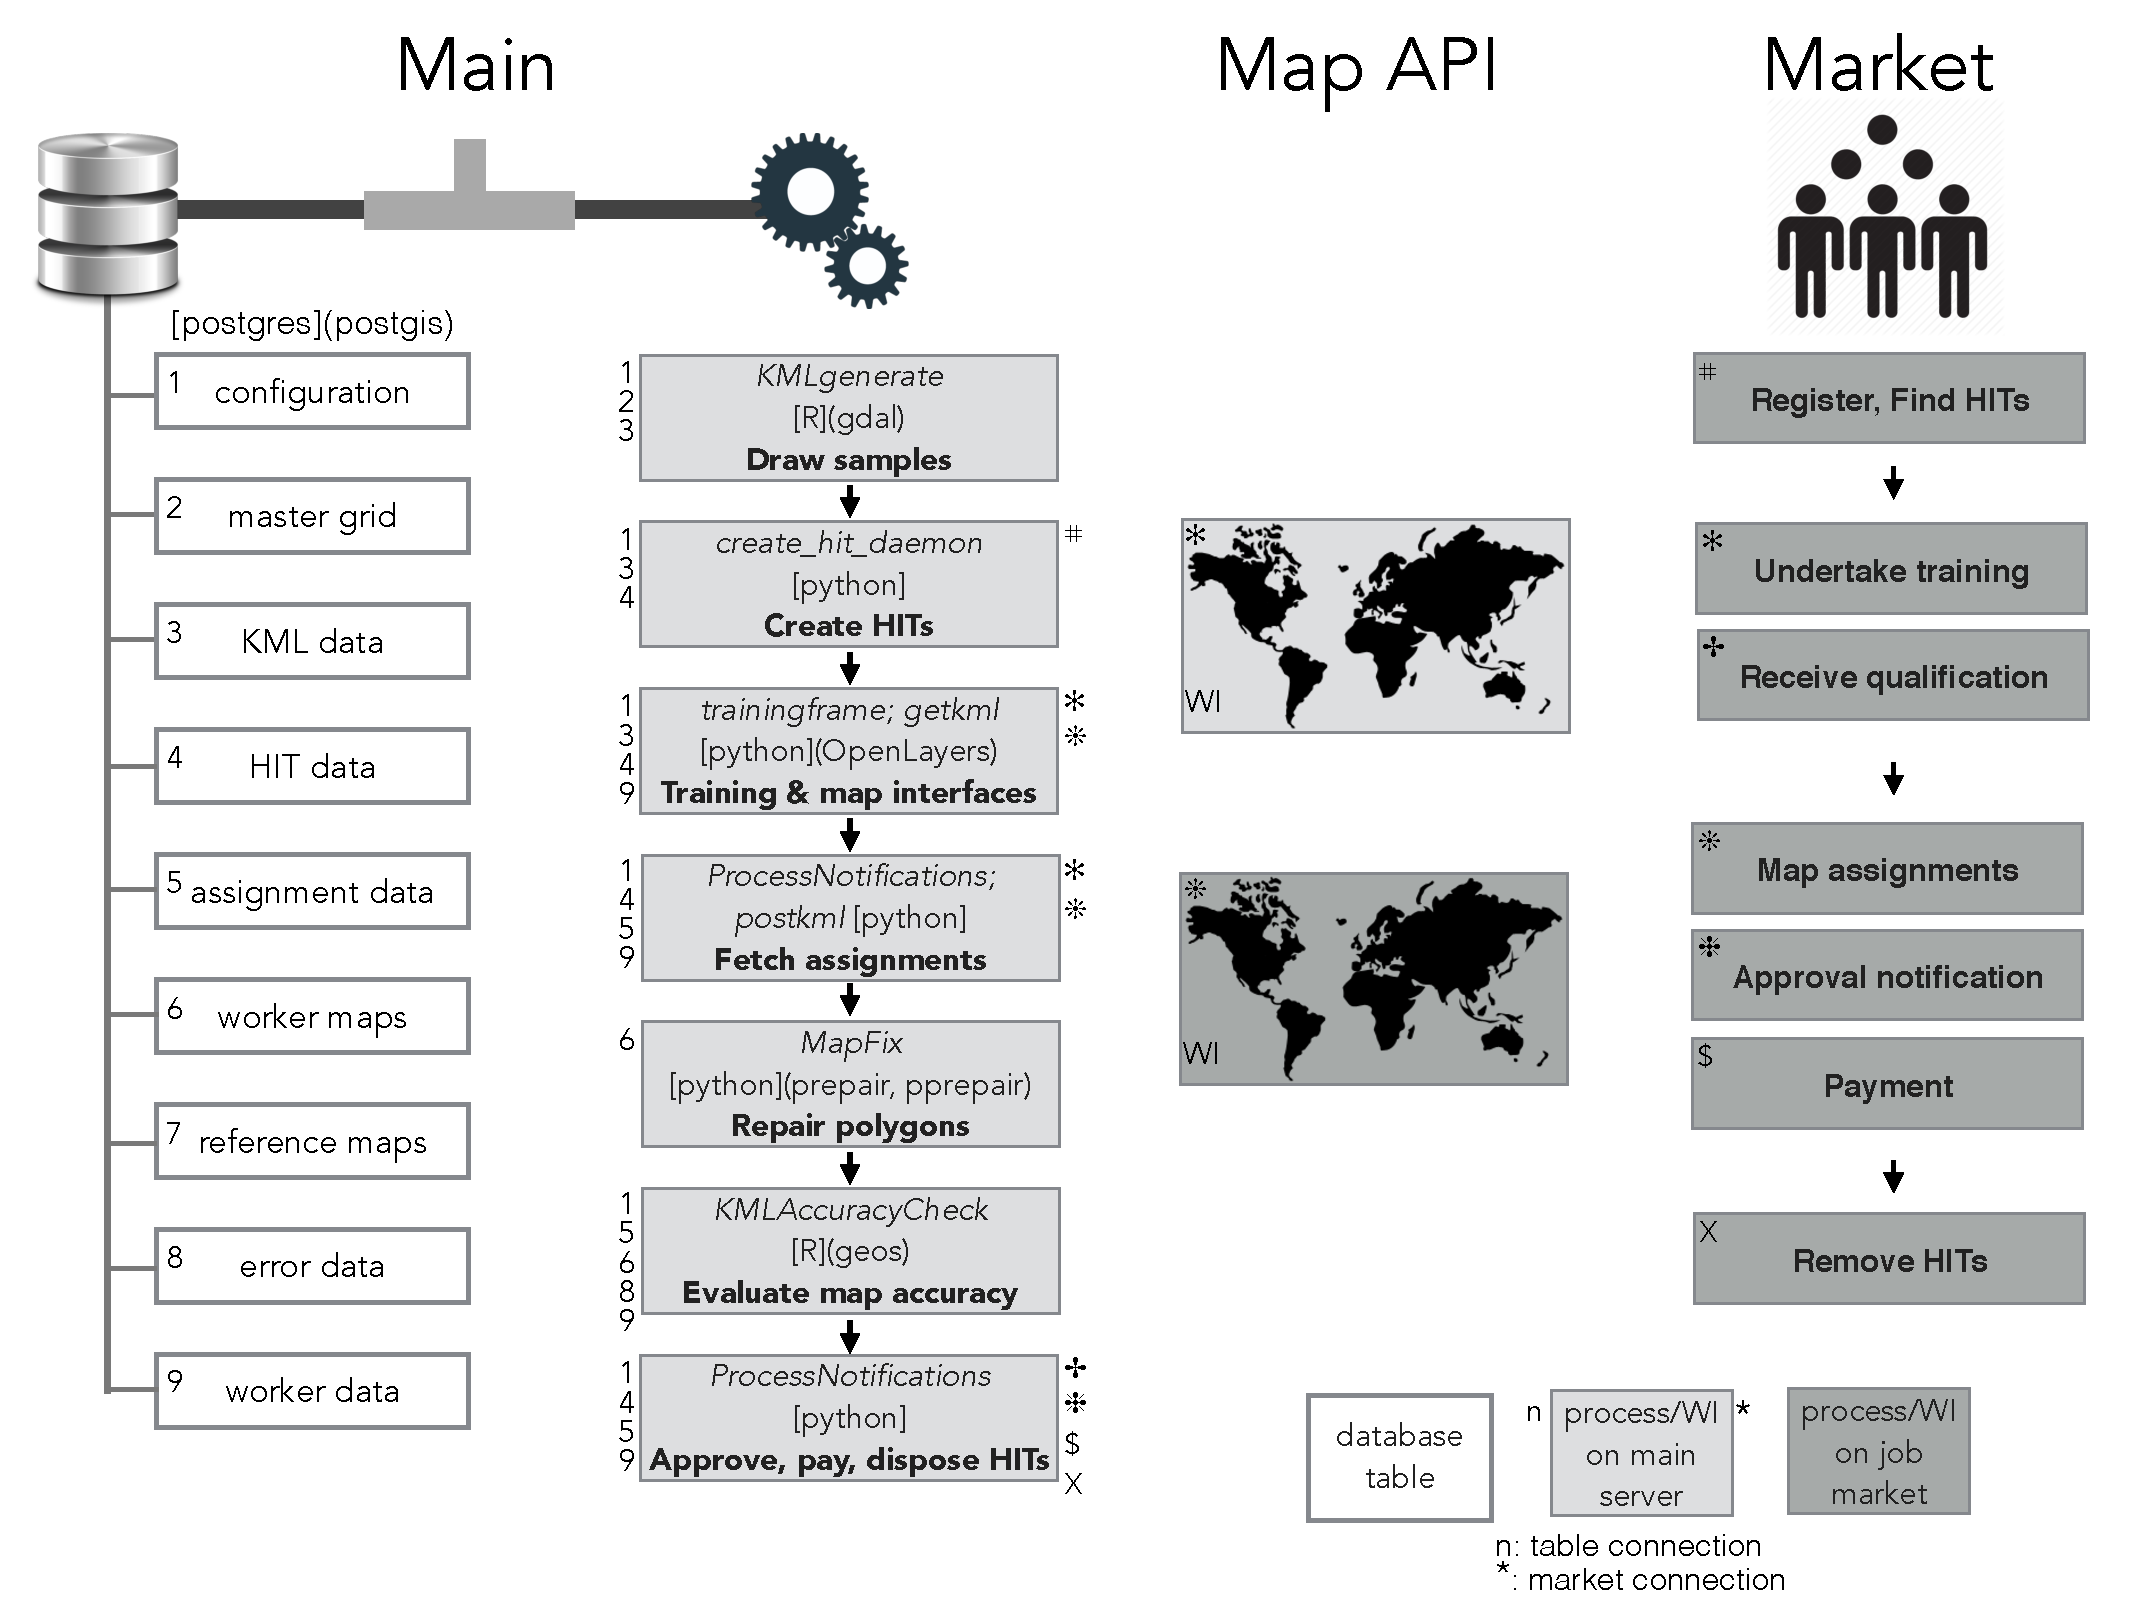
\includegraphics[scale=0.5]{figures/fig2.pdf}
    \caption{The components, and primary processes of DIYlandcover. The main server contains the system database and processes. Primary data tables are shown by the white boxes with grey borders. Primary processes are shown in light grey boxes (process names are italicized, primary software in brackets and its external dependencies in parenthesis, and description in bold). Server processes interact with specific data tables (indicated by the numbers to the left), and with processes that occur in the online job market (indicated by symbols to the right). The two versions (one for training, one for qualified workers) of the worker interface (WI) to the map API are shown, color-coded according to where they are hosted (on main server or online market). }
    \label{default}
  \end{center}
\end{figure}

After the initial random draw (of a user specified size) is taken to identify quality assessment (Q) sites (Section 2, Fig. 1), the selected cells' status is set to unavailable. The geometries are written to individual keyhole markup language (KML) files, and their IDs are added to a ``KML data'' table, where a field specifying cell type is set to "Q" to indicate that the corresponding KMLs reference quality control sites. The user has to provide landcover reference maps for these sites, the geometries of which are stored in a ``reference maps'' table.  

The next draw collects sites that will form the normal (``N'') map production process, where a worker (or workers) creates maps for locations where the underlying landcover is unknown.  This step is governed by \emph{KMLGenerate}, an R process that connects to the database \citep[via the RPostgreSQL package; ][]{conway_rpostgresql:_2012}, takes a weighted random draw of size X (a parameter stored in the ``configuration'' table that holds all variables used by DIYlandcover) from the master grid table, writes each cell geometry to a separate KML file, adds the selected cell IDs to the KML data table, and sets the field type value to ``N". The script changes the cell status in the master grid to unavailable. As N type maps assignments are completed, their status is set to mapped in the KML data table. \emph{KMLGenerate} runs as a daemon, selecting a new random draw as soon as the number of unmapped sites falls below a specified number, ensuring that there is never a system delay in sending mapping assignments to the job market (see 3.2).  

\subsection{Creating mapping assignments}
Following selection, each site is converted into a mapping task for online workers. These tasks are referred to as Human Intelligence Tasks (HITs), in Mechanical Turk's parlance. HITs are created by (\emph{create\_hit\_daemon}), a python daemon that uses the boto library to interface with Mechanical Turk (MT). The daemon polls MT (at regular intervals) to see how many DIYlandcover HITs of types Q and N exist on MT (zero at start of production), and whether they fall below their minimum required numbers. These numbers are calculated from two configuration parameters: the minimum total number of HITs that should be available on MT, and the percentage of these that should be of Q type. If the actual numbers of each type fall below their target numbers, \emph{create\_hit\_daemon} selects the IDs of available KMLs from the KML data table, and sends these together with associated HIT metadata, which includes the pay rate, the number of times the HIT should be mapped, the qualifications required to undertake the HIT (see 3.5), and a definition of the task. MT then registers each HIT and provides it with a unique HIT ID and registration time, which is logged into a ``HIT data'' table on the main server. 

\subsection{Undertaking the mapping assignment}
Once a HIT is registered on MT, it is visible to all workers in the marketplace, but can only be undertaken by qualified workers (see 3.5). Qualified workers who choose to undertake DIYlandcover-generated HITs are first shown a default HIT preview, and they must choose to accept it before they can see the actual location to map. This step helps prevent workers from declining more challenging sites, which bias the sample towards simpler landcovers.

To enable workers to perform a mapping HIT, DIYlandcover uses an OpenLayers interface to the image server, which sits within MT's user screen, centers the map view on the site of the HIT location, and provides a set of digitization tools  (Fig. 3). As soon as the worker accepts the HIT, it becomes a mapping assignment that is issued a unique assignment ID. A Web Server Gateway Interface (wsgi) script, \emph{getKML}, retrieves the OpenLayers javascript, the frame size parameters for the MT interface, the url for the KML demarcating the sample site, and user instructions (e.g. tool use tips), and passes these to MT, and collects the worker, assignment, and HIT IDs and acceptance time, and records these into the ``assignment data'' table. 

The worker then draws polygons around the landcover type(s) of interest that intersect the KML sample square (Fig. 3), and has the option to edit or delete individual geometries and provide comments. On completion, the worker saves the map, and is then taken to the next HIT preview screen. Alternatively, the worker may choose to return the assignment uncompleted. If this happens more than a specified number of times, the worker's qualification can be revoked (see 3.4), which is another check against sample selection bias.  The assignment is automatically abandoned if it is not completed within a defined time. We impose this last restriction to minimize bias in the estimation of wage rates (see 4.2); if workers leave the assignment unfinished on their computer for long periods, the amount of time required to complete assignments will be inflated.

\begin{figure}[!ht]
  \begin{center}
    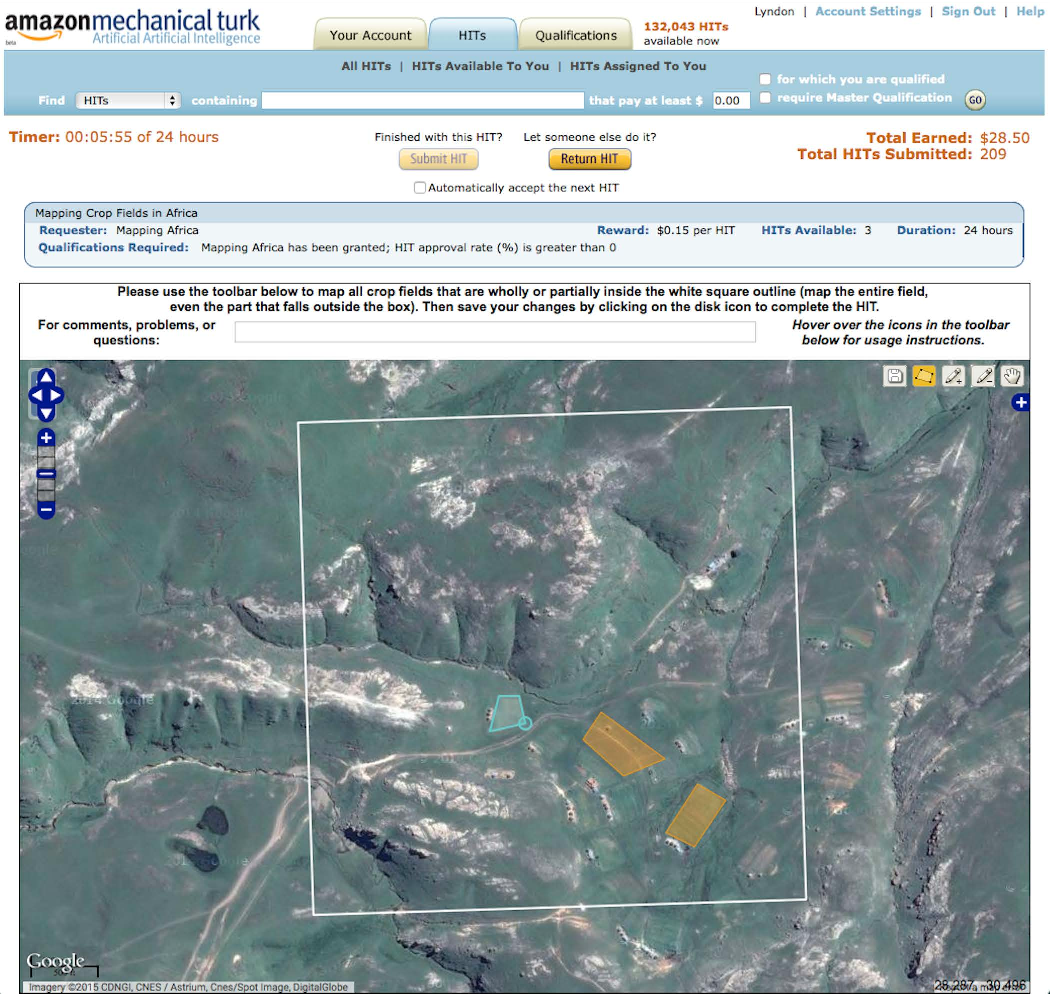
\includegraphics[scale=0.85]{figures/fig3.pdf}
    \caption{The DIYlandcover mapping interface within Amazon.com's Mechanical Turk job marketplace. The white square is the KML sampling frame, gold polygons are completed crop field polygons, the blue polygon is a field in the process of being mapped. Mapping controls are in upper right corner of the image frame.}
    \label{default}
  \end{center}
\end{figure}

When the assignment is completed, returned, or abandoned, MT sends an email notification to the main server, where it is retrieved by \emph{ProcessNotifications}, a python process. If the assignment is returned or abandoned, it is marked as unprocessed and returned to the pool of available HITs on MT, and the worker receives no pay. If the assignment was completed, post-processing routines are triggered. 

\subsection{Processing completed assignments}
Several processing steps must be performed before the worker is paid for the completed assignment, which depend on whether the worker created any polygons during the assignment, and whether it was of Q or N type. If the worker created polygons, then the geometries, KML ID, assignment ID, and completion time are stored in the ``user maps'' data table by process \emph{postKML}, which then triggers \emph{mapFix}, a python script that invokes prepair and pprepair \citep{ohori_validation_2012}, which repair the topologies of single and multi-polygons, respectively. This step is essential because hand-digitized polygon data often contain errors, such as self-intersections and unintended overlaps, which can render topologies invalid and cause subsequent spatial analyses (per 3.4) to fail.  The repaired geometries are then inserted into the user maps table.  

Next, the assignment is given a score, which is recorded in the assignment data table. If the assignment was of N type, this score is null;  for Q type, \emph{KMLAccuracyCheck}, an R process, is called to compare the worker's and reference maps, with the score determined by:

\begin{equation}
  \textrm{S} = \beta_1\textrm{C} + \beta_2\textrm{O} + \beta_3\textrm{I}
%  S = \beta_1\left(1 - \frac{abs(n - N)}{max(n, N)}\right) + \beta_2\frac{a}{a + c} + \beta_3\frac{a + b}{a + b + c + d}
\end{equation}

\noindent Where S is overall mapping accuracy, $\beta_1$-$\beta_3$ are user-defined weights, and: 

\begin{equation}
  \textrm{C} = 1 - \frac{\textrm{abs}(\textrm{n} - \textrm{N})}{\textrm{max(n, N)}}
\end{equation}
 
\begin{equation}
  \textrm{O} = \frac{\textrm{a}}{\textrm{a + c}}
\end{equation}

\begin{equation}
 %\textrm{inside} = \left( \frac{\textrm{a + b}}{\textrm{a + b + c + d}}\right)  \vert  \left(\frac{\textrm{a}}{\textrm{a + c}} + \frac{\textrm{d}}{\textrm{b + d}} - 1\right)
 \textrm{I} = \frac{\textrm{A + D}}{\textrm{A + B + C + D}}
\end{equation}

Or: 

\begin{equation}
  \textrm{I} = \left(\frac{\textrm{A}}{\textrm{A + C}} + \frac{\textrm{D}}{\textrm{B + D}}\right)0.5
\end{equation}

\noindent With C being count error, or the agreement between the number of landcover polygons in the worker's maps (n) and in the reference data (N). O measures map agreement for those parts of the worker's and reference polygons that fall \emph{outside} of the KML grid, where a is the area of overlap, and c is the false negative error (i.e. the area of reference field polygons falling outside the grid that the worker failed to map). I measures map accuracy \emph{inside} the KML grid, with A being the grid interior equivalent of a, B the false positive error (i.e. landcover incorrectly labelled by the worker), C the false negative error (landcover area missed by the worker), and D the true negative area (area correctly left unmapped). I can be calculated using standard classification accuracy (Eq. 4), or a variant of the True Skill Statistic \citep[Eq. 5][]{allouche_assessing_2006}, a more stringent measure that corrects for class prevalence, which we compressed to fall between 0 and 1 rather than -1 to 1. The areas of a, c, A, B, C, D are calculated using intersection and difference operations provided by the rgeos library \citep{bivand_rgeos:_2013}, after transforming maps to a projected coordinate system.  

We include the O metric to encourage workers to completely map features intersecting the sampling grid (i.e. either falling entirely within or both within and outside of it), in order to have unbiased estimates of landcover size classes. However, we can only partially assess the accuracy of exterior features because it is impossible to correctly define negative space outside the sample grid, since it is both unbounded and may contain target features that will not be mapped because they do not intersect the grid. An error map showing each of the accuracy assessment components is illustrated in Figure 4.

\begin{figure}[!ht]
  \begin{center}
    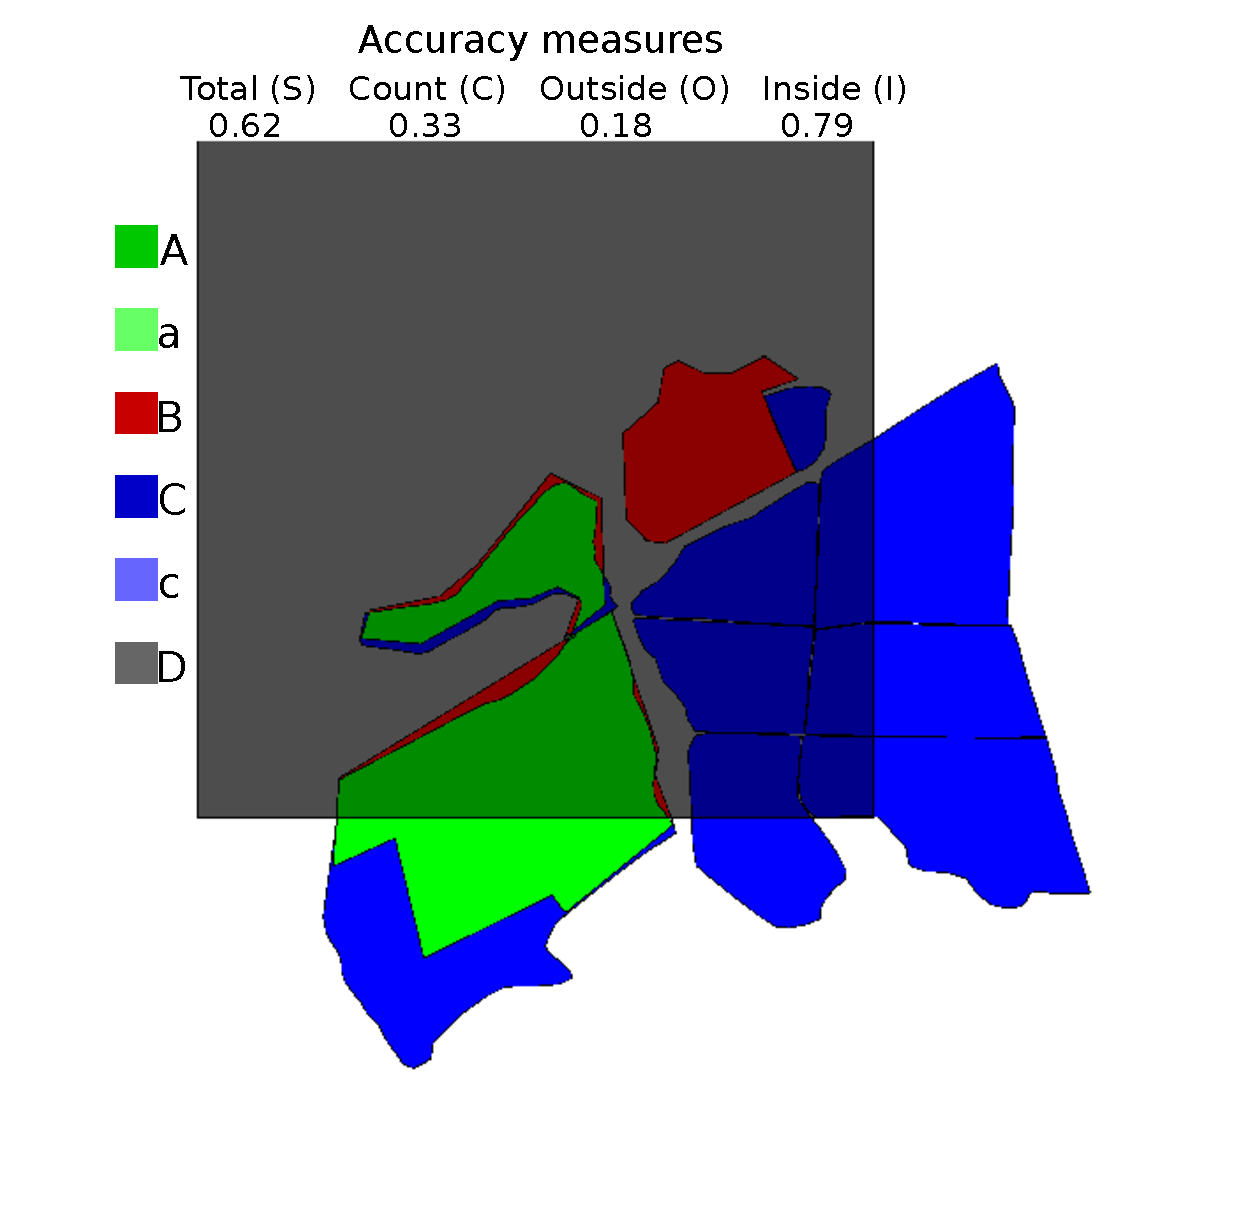
\includegraphics[scale=0.8]{figures/fig4.pdf}
    \caption{A graphical illustration of the accuracy assessment algorithm (as applied to cropland maps), providing the resulting scores for overall accuracy (Eq. 1) and count, outside, and inside error (Eqs. 2-5), where each component ranges between 0 (most error) and 1 (no error). The area of each error component is color-coded: A (agreement inside the grid), a (agreement outside), B (false positive error inside the grid), C (false negative inside), c (false negative outside), and D (true negative inside). }
    \label{default}
  \end{center}
\end{figure}

Once the algorithm has run, all accuracy measures (S, C, O, I) are stored in the ``error data'' table, while S is stored in the assignment data table. S is also added to a vector of Q scores for the specific worker (stored in the ``worker data'' table), which is used to calculate a moving average of the worker's recent performance.  If S is above a minimum accuracy threshold, then the assignment is approved. If rejected, then payment is withheld, and a notice is sent to MT where it is added to the worker's system-wide rejection rate. Successive rejections can result in the revocation of mapping qualifications if a worker's \emph{quality} score drops below the accuracy threshold. The quality score is:

\begin{equation}
  \textrm{quality} = \frac{{\textrm{S}_{\textrm{i}} + \textrm{S}_{\textrm{i-1}} + ... + \textrm{S}_\textrm{i-(j-1)}}}{j} - \beta_4\frac{{\textrm{R}_{\textrm{i}} + \textrm{R}_{\textrm{i-1}} + ... + \textrm{R}_\textrm{i-(j-1)}}}{j}
\end{equation}

Where i is the most recent S value calculated, and j the total number of recent S scores to use in calculating a mean S. To minimize assignment selection bias (see 3.3), an additional penalty, the worker's rate of assignments accepted but returned without completing (R, which equals 1 for a return, 0 for a completion), is multiplied by a weight $\beta_4$ and deducted.  

In cases where the worker returns no maps for a Q type assignment, map storage and cleaning does not occur before \emph{KMLAccuracyCheck} is run. In these cases, the C and O scores (Eq. 2 \& 3) reduce to 1 where the reference map has no landcover polygons, or 0 if it does. If the assignment is of N type, it is scored as NULL and added to the assignment data table.  

Unlike the Q type, N assignments are automatically approved, under the logic that the worker's quality score at the time of map creation is indicative of that map's accuracy. The exception to this is N assignments created by a newly qualified worker (see 3.5), which are marked as ``untrusted'' in the assignment data table until that worker completes as many Q assignments as are needed to calculate the moving average accuracy score. Upon assignment approval, \emph{ProcessNotifications} relays a message to MT and the worker is paid (see 3.6) from the Requester's account, and then removes the corresponding HIT from MT. Q sites will be re-created as HITs multiple times, while N sites are mapped just one time.

%\begin{table}[htdp]
%\caption{default}
%\begin{center}
%\begin{tabular}{|c|c|}

%\end{tabular}
%\end{center}
%\label{default}
%\end{table}%

\subsection{Worker qualification and payments}
All workers performing mapping assignments must first be qualified, which is treated as a special case of Q type assignments. MT evaluates the qualification status of each worker attempting to access a DIYlandcover HIT. If the worker is not qualified, a link to a training module is presented on the MT interface. The module, which is hosted on the main server, is managed by \emph{trainingframe}, a python process, which issues each new trainee a unique training ID. The trainee first watches video tutorials explaining the project and its mapping rules, and is then required to map several training sites, the accuracy of which is assessed by \emph{KMLAccuracyCheck}. Trainees must map each site to the minimum accuracy standard, but are given unlimited chances to do so. A separate set of tables mirroring those used for collecting map, assignment, worker, and error data is used to record training data. Once a worker successfully completes all training sites, a qualification request is posted on MT.  A daemon, \emph{process\_qualifications\_requests}, polls MT at specified intervals, collects these requests together with associated worker and training IDs, examines for each worker whether all training sites were completed successfully, and, if so, adds the trainee's worker ID to the worker data table, sets the qualification status to true, then sends a notice to MT that the worker is now qualified. Candidate workers who fail to pass all training sites, or workers whose qualifications are revoked due to poor accuracy (see 3.4), can repeat the training to qualify/re-qualify. 

%Each worker who attempts to access a The ID of each worker who attempts to access a DIYlandcover HIT is compared against the worker data table by\emph{ProcessNotifications}. If the worker's ID is not found, a link to a training module is presented on the MT interface.

Upon qualification, workers are paid a small bonus, and can begin mapping assignments. Workers are paid a flat rate for approved assignments. To incentivize worker performance, DIYlandcover also allows bonus payments to be made based on the worker's accuracy score. If implemented, the bonus algorithm, managed by \emph{ProcessNotifications}, pays an extra per assignment amount if the worker's quality score exceeds certain thresholds.

\section{Applying DIYlandcover to map South African crop fields}
We examined the capabilities of DIYlandcover by applying it to map crop field boundaries in South Africa. We selected South Africa because its cropland is already mapped \citep[see section 2;][]{geoterraimage_south_2008}, which provided us with a readily adaptable set of reference maps, and it has a broad mix of agricultural systems that is representative of the image interpretation challenges facing workers. This mix ranges from hard to detect communal and smallholder agriculture, to more easily discerned industrial fields \citep{hardy_rainfed_2011}. The application of DIYlandcover in South Africa also provides the test site for the \href{http://mappingafrica.princeton.edu}{Mapping Africa} project, which aims to create high quality cropland maps for sub-Saharan Africa. 

\subsection{Mapping set-up}
We created a 1X1 km, Albers Equal Area Conic-projected sampling grid for South Africa, and created a logistic regression model to define the probability of cropland presence throughout the country. We used a randomly selected subset of field centroids from the existing cropland data as the positive response case, and an equal sized draw of the non-croppred areas as the negative case. We used a gridded rainfall surface, a digital-elevation model derived measure of topographic roughness, and a map of protected area boundaries as predictor variables \citep[for further details on these variables and see][]{estes_comparing_2013,estes_using_2014}. We divided the resulting probability into quartiles, which provided the weights used by \emph{KMLGenerate}.

For Q sites, we drew 609 grid cells (0.05\% of South Africa's area), and intersected these with the polygons in the existing cropland data to create the associated Q data tables (3.1). We then further edited these polygons so that our Q maps would be consistent with the imagery in the Google Maps API, and to conform with the specific mapping rules that we set for workers (Table 1); we asked workers to map sites where crop fields were actively or very recently (e.g. within the past 2-3 years) used for arable agriculture. Longer term fallows or abandoned fields, permanent crops (orchards, commercial afforestation) were to be left unmapped, in which case workers simply saved the assignment. In cases of uncertainty (e.g. the worker had trouble telling whether the field was active or abandoned), workers were asked to map every second instance.  

\begin{table}[htdp]
  \caption{Rules for mapping crop fields in South Africa-focused application of DIYlandcover. Workers were asked to map only currently active (i.e. farmed within the past 2-3 years) annual crop fields, and to not delineate other agricultural types.}
   \begin{center}  
   \begin{tabular}{l|l}
      \hline
      \textbf{Feature type} & \textbf{Action} \\
      \hline\hline
      No cropland visible & Don't map \\
      Active annual crop field & Map \\
      Fallow crop field & Don't map \\
      Unsure if active crop fields & Map every second feature \\
      Orchards & Don't map \\
      Afforestation & Don't map \\
      Pastures & Don't map \\
     \hline
  \end{tabular}
  \end{center}
  \label{default}
\end{table}%

For N sites, we established 500 as the minimum number of KMLs that should be available on the main server, and 10 as the minimum number of HITs to maintain on MT, of which 20\% should be Q type (meaning workers had a 1:5 chance of mapping a Q site). MT was polled every 10 seconds to see if new HITs were needed.   

The accuracy algorithms (Eq. 1) $\beta$ terms were set as 0.1, 0.2, and 0.7 for the C (Eq. 2), O (Eq. 3), and I terms (here Eq. 4). We selected a low weight for C because determining the boundaries of individual fields from overhead imagery is fairly subjective, even for expert observers, and we did not want to unduly penalize workers for a difference in judgement, yet we also wanted to discourage rapid mapping that erased boundaries between clearly distinct fields. We gave O a slightly larger weight to stress the importance of completed fields that extended outside the sample grid, but a larger weight would give the worker too much credit for cases where no fields intersected the grid. The I term was weighted most heavily because it is the only place where workers' abilities to correctly distinguish null space can be assessed.  We used the same weights to assess assignments within the 8-site training module.       

Payment was set at \$0.15 per assignment. A four-tier bonus payment algorithm was also written into logic. We did not implement this logic in our initial trial, in order to first assess whether the base rate would allow workers to achieve our target wage of \$8-10 hour$^{-1}$, but we evaluated the cost implications of bonus payments set to \$0.01, \$0.02, \$0.03, and \$0.05 for worker quality scores exceeding 0.85, 0.95, 0.975, or 0.99, respectively. 

\subsection{Trial results}
The Mapping Africa trial ran on Mechanical Turk for 26.4 hours between October 2-3, 2013, resulting in 945 mapping assignments, of which 882 were approved, 10 were rejected (due to failing accuracy scores), and 53 were not completed (i.e. returned or abandoned).  A total of 707 N sites with 216 (31\%) containing worker-delineated polygons were mapped, as well as 185 Q sites, with 65 (35\%) having fields (Fig. 5). 

\begin{figure}[!ht]
  \begin{center}
    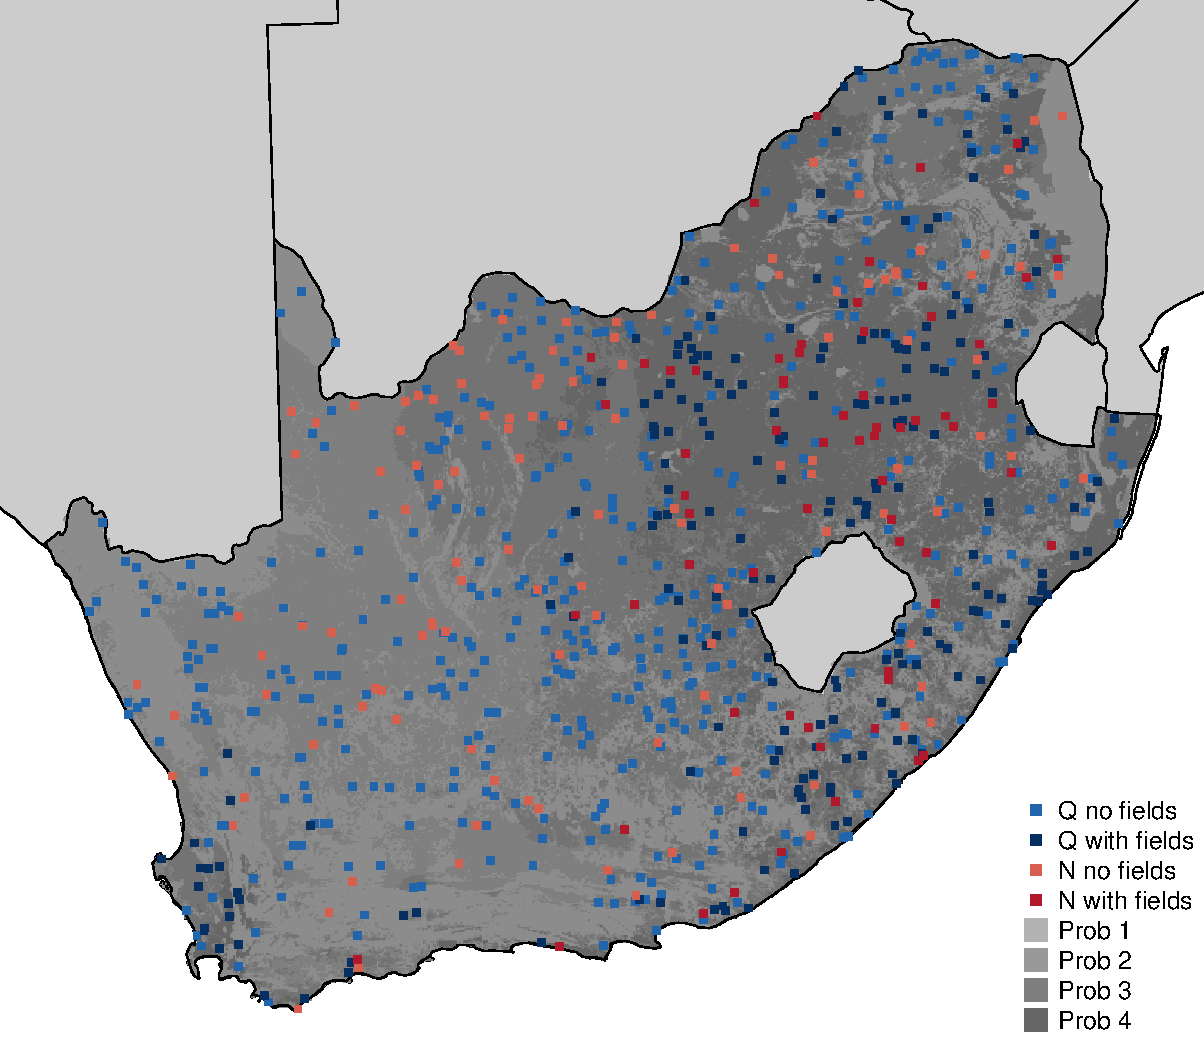
\includegraphics[scale=0.7]{figures/fig5.pdf}
    \caption{A map of DIYlandcover trial results over South Africa, showing the distribution of mapped sites, color-coded according to their assignment type (Q or N) and whether they contained worker-mapped crop field boundary polygons. The grey shading indicates the four-category weighting derived from a logistic regression model of cropland occurrence.}
    \label{default}
  \end{center}
\end{figure}

These sites were mapped by 15 different workers, from a pool of 18 who passed the initial qualification test. A further 18 took the qualification test but failed to pass. The distribution of mapping effort was highly skewed, with three workers completing 65\% of the total assignments (Fig. 6A).  The average Q:N assignment ratio for each worker was 18\%, but there was high variability among workers who completed less than 50 assignments (Fig. 6A). The mean accuracy assessed across all Q sites (using Eq. 1 with Eq. 4) was 0.91 (out of 1), but Q sites containing fields were mapped with lower accuracy (0.79) than sites without fields (0.97; Fig. 6B). To understand this discrepancy more fully,  the number of polygon vertices in the reference polygons can be used as proxy for cropland complexity, and thus assignment difficulty.  Worker accuracy declined significantly, albeit weakly (p$<$0.048), in relation to this complexity (Fig. 6C). Worker effort also declined strongly as a function of map complexity (Fig. 6D); the more fields there were to map---or the more intricate their boundaries---the fewer vertices placed by workers, presumably to minimize mapping time. This reduction in effort may partially explain the increased error. 

\begin{figure}[!ht]
  \begin{center}
    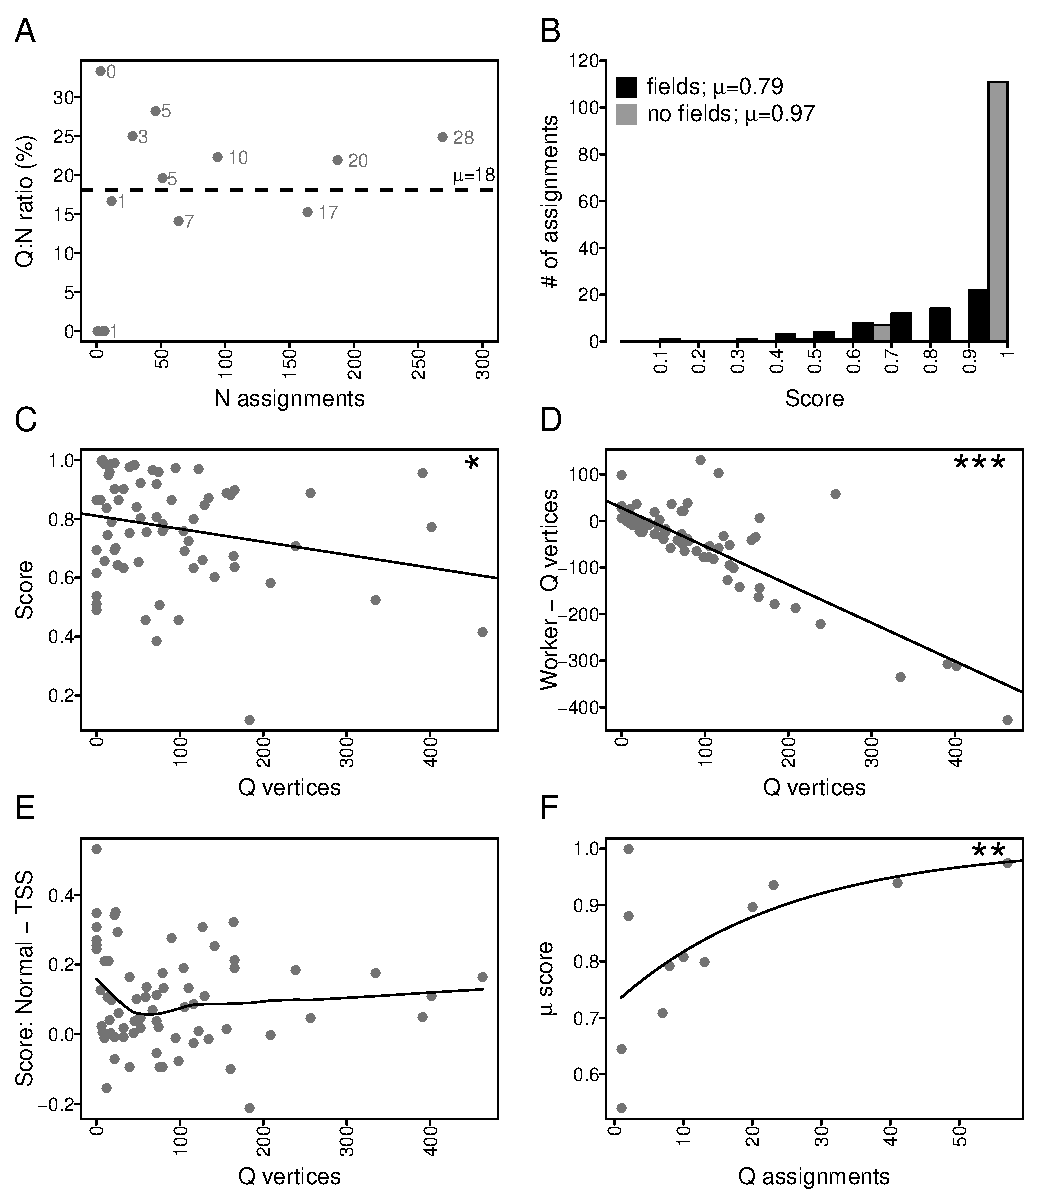
\includegraphics[scale=0.66]{figures/fig6.pdf}
    \caption{Results from initial DIYlandcover trial, including A) the total number of completed assignments per worker versus the ratio of Q to N type assignments (values in grey next to points represent the percent of total assignments); B) the distribution of accuracy scores segregated by assignment type (black bars = Q type, grey bars = N type); the number of vertices in reference map polygons versus C) accuracy score, D) the difference between the number of vertices in workers' and reference map polygons, and E) the difference between accuracy scores calculated using Equation 4 or Equation 5 (the True Skill Statistic); F) the number of Q assignments completed by each worker versus worker mean accuracy score. Significance of regression fits in C, D, F are:  $\ast$p$<$0.05; $\ast$$\ast$p$<$0.01; $\ast$$\ast$$\ast$p$<$0.001. C and D are linear models, F is asymptotic regression.} 
    \label{default}
  \end{center}
\end{figure}

Replacing Equation 4 with Equation 5 (the True Skill Statistic; TSS), which corrects for class prevalance  \citep{allouche_assessing_2006}, to calculate map score (Eq. 1) removed the significant negative relationship between map score and complexity (F-statistic: 1.54; p$<$0.22). At sites with only a few fields, which are both less complex and typically having a much higher share of non-cropped than cropped area, Eq. 4 was more lenient than at more complex sites, because the worker received proportionally more credit for ``mapping'' the uncropped space.  This tendency is seen in Fig. 6E, which indicates that the Equation 4 variant was generally more positive than the Equation 5 variant (on average 0.1 higher for sites with fields), but particularly so where truth maps had fewer than 25-50 vertices (0.14-0.12 higher).

Accuracy appears to improve with experience, as workers' average accuracy scores increased in proportion to the number of Q assignments completed. Accuracy gains increased rapidly below 20-25 completed Q assignments, and then leveled between 0.9 and 1 (Fig. 6F).  

%N sites per worker
%Accuracy
%Accuracy per worker
%Accuracy as function of vertex density 
%Accuracy as function of time/experience

We paid \$132.30 to workers for the 882 approved assignments, with a total cost to the project of \$145.53 after accounting for Amazon.com's 10\% Requester surcharge. Of this, \$28.88 was paid for the 175 approved Q assignments and \$116.66 for the 707 N assignments.  Our post-hoc application of the bonus algorithm, which requires workers to complete at least five Q assignments (8 of 15 met this requirement), would have added \$21.89 (15\%) to the trial's cost. 

To examine the effective worker wage, we divided total pay by the mean assignment duration, which we calculated as  the difference between assignment acceptance and completion times. Since workers could accept assignments without immediately completing them (maximum assignment duration was 24 hours), we can not precisely measure mapping time. However, our experience suggests that the most complicated sites require $<$30 minutes of mapping effort, thus we excluded any assignments that took longer from the wage calculations. The resulting mean wage across all workers was \$11.50 hr$^{-1}$. For sites where fields were mapped, the effective wage was \$3.89 hr$^{-1}$, and for sites without fields it was \$14.07 hr$^{-1}$.  Factoring in bonus payments, wages would have been \$12.33 overall, \$4.18 for sites with fields, and \$15.19 for sites lacking fields. 

The flat rate cost to map a single square kilometer was \$0.165, including the cost of accuracy assessment and Amazon.com's fees, or \$0.19 had we included bonus payments. At these rates, the cost of mapping South Africa in its entirety (1,219,095 1 km$^2$ cells) would be \$201,151-231,407, or \$3.4-3.9 million for all of non-Saharan Africa (20.8 million km$^2$). 

\section{Discussion}
The initial trial demonstrates that DIYlandcover can be an effective platform for generating landcover data that is of higher quality than conventional landcover products. This quality is attributable to humans' well-known superiority in classifying landcover types, which is supported by the fact that expert image interpretation is a key component of training and assessing existing landcover mapping algorithms \citep[e.g.][]{fritz_cropland_2011,fritz_geo-wiki:_2012,hansen_high-resolution_2013}. Here we found that workers with less than 24 hours of mapping experience were able to map cropland with 91\% accuracy. Although accuracy and mapping precision decreased when sites contained crop fields, and in proportion to the complexity of those fields (Fig. 6), the overall accuracy is higher than the latest generation landcover dataset of comparable resolution \citep[82\%;][]{fritz_mapping_2015}. This comparison may also underestimate DIYlandcover's accuracy, as the algorithm we use evaluates all four accuracy components (true and false positives and negatives) at \emph{each} mapped site (see Fig. 6B), making it more sensitive than conventional measures of landcover map accuracy, which are calculated \emph{across} all sites. The positive relationship we see between worker experience and score (Fig. 6F) also suggests that DIYlandcover's accuracy improves with time, although this needs to be re-evaluated after a lengthier period of operation, as does the affect of the different accuracy component weights (Eq. 1) in terms of influencing worker--and thus system--performance. 

Beyond classification accuracy, the geometric detail captured in workers' maps is an additional dimension of data quality that is lacking from current landcover products. Such extra information on landcover pattern may be useful for predicting important social, economic, and environmental processes \citep{fritz_mapping_2015}.   

The trial also suggested that DIYlandcover can generate map data rapidly, given that a relatively large number of workers undertook assignments relative to the short operational window.  Extrapolating linearly from the rate new workers qualifying (0.7 hr$^{-1}$), there would be 235 qualified workers within two weeks, who would complete a wall-to-wall map of South Africa in 110 days, assuming they mapped at the average observed rate of 59 km$^2$ worker$^{-1}$ dy$^{-1}$ (including the proportion of Q assignments). This speed could be comparable to that of automated landcover classification, when factoring in the cycle of image pre-processing and algorithm training, testing, and implementation.  

It is not unreasonable to think that this mapping speed could be met or exceeded, given a wage comparable to the one we used here, which was much greater than the estimated average \$2 hr$^{-1}$ received by Mechanical Turk workers \citep{marvit_how_2014}. We chose this rate because our HITs were more complicated than those typically requested on MT, and also because we did not want DIYlandcover to contribute to worker exploitation, which is a growing concern about crowdsourcing \citep{marvit_how_2014}. 

Higher wages naturally increase the cost of landcover maps. Although we argue that several million dollars would be a small price to pay for an accurate, Africa-wide map of crop field boundaries, these sums are well beyond the reach of most research budgets. Several methodological improvements could help mitigate these costs. The first is to redesign base payments to be proportional to mapping effort. In the case of crop fields, payments could be scaled to match field density and complexity. This could be achieved by using more accurate cropland probabilities to stratify site selection. These probabilities could be provided by the latest cropland percentage map \citep{fritz_mapping_2015}, which should be far more informative of likely mapping effort than the simple logistic regression surface we used. Sites with low cropland probabilities would be paid a very small amount (\$0.01) whereas high probabilities sites might be paid  (e.g. \$0.5-1.00). Creating more weight categories (e.g. 10 instead of 4) would allow the sampling scheme to be more precisely targeted towards cropland. The combination of these two changes could allow more cropland to be mapped for the same cost (provided the tiered rates are calibrated to the wage target), with the added benefit that appropriate pay rates might remove the negative relationship between worker precision and map complexity (Fig. 6D). Using the stricter version of the accuracy score, together with bonus payments, may also incentivize greater effort for such locations.   

Other improvements could be made to minimize researcher's time costs, particularly with respect to generating reference maps. Our trial reference maps took several weeks to digitize, and were based on the judgement of a few people. Creating our reference data was thus both time-consuming and somewhat subjective. A third type of mapping HIT, one that would allow repeated mapping by multiple workers, could help to overcome these two problems. The resulting maps could be combined to create a more robust ``truth'' based on between-worker agreement, as illustrated by the combined maps from the eight qualification sites used in the trial (Fig. 7). This approach could greatly minimize the time required to develop reference data, and we suspect that the consensus maps of many workers (which could be weighted based on worker quality scores) will be more accurate than those of one or two experts. The last assumption still needs to be verified against field-collected landcover data.   

\begin{figure}[!ht]
  \begin{center}
    \includegraphics[scale=0.78]{figures/fig7.pdf}
    \caption{The eight sites used in the South Africa trial qualification test. Columns 1 and 3 show the unmapped imagery; columns 2 and 4 display the combined maps of all 19 trainees.  Map colors indicate the fraction of trainee maps that overlap. } 
    \label{default}
  \end{center}
\end{figure}

These measures would still be insufficient to make creating spatially comprehensive, large area maps affordable for most researchers. If it is to be affordably used for this purpose, DIYlandcover should be ported to a server that supports voluntary crowdsourcing efforts, similar to the Geo-Wiki project \citep{fritz_geo-wiki:_2012}. The question then is how long it would take volunteer workers to map the designated area. An alternative, more advanced, application would be to use DIYlandcover to train and test newer computer vision approaches for mapping noisy landcover types, such as smallholder crop fields \citep[e.g.][]{debats_generalized_????}. In this case, DIYlandcover would work iteratively with the algorithm until an acceptable level of accuracy is achieved, with site selection weighted towards areas of greatest classification error after each step. This approach could strike the best balance between cost, mapping speed, and accuracy, as it would harness the complementary strengths of human (more effective at recognizing patterns in noisy RGB or black and white images) and computer image classifiers (able to extract patterns in high dimensional data, such as multispectral imagery, which are hard for humans to interpret).  An alternative possibility for this use case---where DIYlandcover validates broader-scale methods---would be test and refine the judgement-based size class estimates created under the Geo-Wiki project \citep{fritz_mapping_2015}. DIYlandcover is highly complementary to this methodology, given its emphasis on precisely measuring landcover geometries.   

DIYlandcover thus appears to offer substantial promise for improving landcover maps. Its first task will be to delineate smallholder fields in southern and East Africa, where it will be used to track cropland changes and constrain Landsat-driven crop yield models \citep{sibley_testing_2014}, and also to develop pattern-based predictors of socio-economic characteristics. It may also be adapted to map a wide range of other discrete landcover types, include burn scars, savanna tree crowns, small water bodies, termitaria, and buildings.  

\section*{Acknowledgements}
This work was supported by funds from the Princeton Environmental Institute Grand Challenges program, the NASA New Investigator Program (NNX15AC64G), and the National Science Foundation (SES-1360463 and BCS-1026776).   

\section*{Supplementary materials}
Supporting figures S1 and S2 are found in AppendixS1; Appendix S2 contains the R code used to analyze trial results and create related figures. 
%\label{}

%% The Appendices part is started with the command \appendix;
%% appendix sections are then done as normal sections
%% \appendix

%% \section{}
%% \label{}

%% If you have bibdatabase file and want bibtex to generate the
%% bibitems, please use
%%
\section*{References}
\bibliographystyle{elsarticle-harv2} 
\bibliography{main}

%% else use the following coding to input the bibitems directly in the
%% TeX file.

%\begin{thebibliography}{00}
%
%%% \bibitem[Author(year)]{label}
%%% Text of bibliographic item
%
%\bibitem[ ()]{}
%
%\end{thebibliography}
\end{document}

\endinput
%%
%% End of file `elsarticle-template-harv.tex'.
